\documentclass[../main-manifolds.tex]{subfiles}

\begin{document}
\providecommand{\szz}{\mathcal{S}}
\providecommand{\ccinf}{C_c^\infty}

% Topologies
\providecommand{\Taux}{\Tau_\xx}
\providecommand{\Tauy}{\Tau_\yy}
\providecommand{\Tauxy}{\Tau_{\xx\times\yy}}

% Basis
\providecommand{\Bx}{\borel_\xx}
\providecommand{\By}{\borel_\yy}
\providecommand{\Bxy}{\borel_{\xx\times\yy}}


\fchapter{A: Review of Topology}
\problem{Properties of Compact Spaces}
\begin{wts}\label{lee-appendix-A.45}
Let $\xx$ and $\yy$ be topological spaces.
\begin{enumalpha}
    \item If $F\in C(\xx,\yy)$, and $\xx$ is compact, then $F(\xx)$ is compact.
    \item If $\xx$ is compact and $F\in C(\xx,\real)$, then $F(\xx)$ is bounded, and $F$ attains its supremum and infimum on $\xx$.
    \item A finite union of compact subspaces of $\xx$ is again compact.
    \item If $\xx$ is Hausdorff, and $A$, $B$ are disjoint, compact subspaces of $\xx$, there exists open $U$ and $V$ st
    \begin{figure}[htbp]
        \centering
        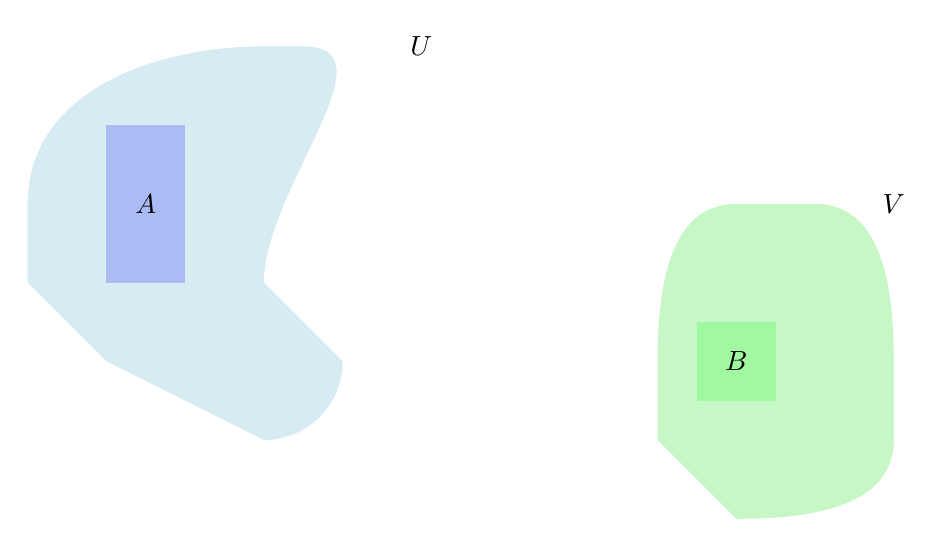
\begin{tikzpicture}
            % Define colors
            \definecolor{lightblue}{RGB}{173,216,230}
            \definecolor{lightgreen}{RGB}{144,238,144}
    
            % Draw the open set U
            \fill[lightblue,opacity=0.5] (1,1) -- (1,2) to[out=90,in=180] (4,4) -- (4.5,4) to[out=0,in=90] (4,1) -- (5,0) to[out=-90,in=0] (4,-1) -- (2,0) -- cycle;
            \node at (6,4) {$U$};
    
            % Draw the closed set A
            \fill[blue,opacity=0.2] (2,1) rectangle (3,3);
            \node at (2.5,2) {$A$};
    
            % Draw the open set V
            \fill[lightgreen,opacity=0.5] (9,-1.2) -- (9,0) to[out=90,in=180] (10,2) -- (11,2) to[out=0,in=90] (12,0) -- (12,-1) to[out=-90,in=0] (10,-2) -- (9,-1) -- cycle;
            \node at (12,2) {$V$};
    
            % Draw the closed set B
            \fill[green,opacity=0.2] (9.5,-0.5) rectangle (10.5,0.5);
            \node at (10,0) {$B$};
        \end{tikzpicture}
        \caption{Closed sets $A$ and $B$ within open sets $U$ and $V$, respectively.}
        \label{lee-appendix-A.45-graphic}
    \end{figure}
    \item Every closed subset of a compact space is compact.
    \item Every compact subset of a Hausdorff space is closed.
    \item Every compact subset of a metric space is bounded.
    \item Every finite product of compact spaces is compact.
    \item Every quotient of a compact space is compact.
\end{enumalpha}
\end{wts}
\newpage
\begin{proof}[Proof of \Cref{lee-appendix-A.45} Part A]
    Let $f\in C(\xx,\yy)$ with $\xx$ compact. Fix an open cover of $f(\xx)$ in the relative topology, 
    \[
        \{U_\alpha\cap f(\xx)\}_{\alpha\in A}\text{ covers }\xx,\: U_\alpha\text{ open in }\yy
    \]    
    So that $\bigcup f^{-1}(U_\alpha) = \bigcup f^{-1}(U_\alpha\cap f(\xx))=\xx$. Since $\{f^{-1}(U_\alpha)\}_{\alpha\in A}$ is an open cover for $\xx$, this induces a finite subcollection of indices $\{\alpha_1,\ldots,\alpha_n\}$ with
    \[
        \bigcup_{j=1}^nf^{-1}(U_{\alpha_j}) = \bigcup_{j=1}^nf^{-1}(U_{\alpha_j}\cap f(\xx))
    \]
    The direct image commutes with unions, therefore
    \[
        f(\xx)=f\biggl(\bigcup_{j=1}^nf^{-1}(U_\alpha\cap f(\xx))\biggr) = \bigcup_{j=1}^nf\biggl(f^{-1}(U_{\alpha_j})\biggr) = \bigcup_{j=1}^n U_{\alpha_j}
    \]
\end{proof}


\begin{proof}[Proof of \Cref{lee-appendix-A.45} Part B]
    Let $\xx$ be compact, and $f\in C(\xx,\real)$, so that $f(\xx)\subseteq\real$ is compact. Compact subsets are closed and bounded in $\real$, let $A = \sup f(\xx)$ and $B = \inf f(\xx)$. Both $A$ and $B$ are accumulation points of $f(\xx)$, so $A = f(x)$ and $B = f(y)$ for some $x$, $y$ in $\xx$.
\end{proof}


\begin{proof}[Proof of \Cref{lee-appendix-A.45} Part C]
    Let $\xx$ be a topological space, and $K_1,\ldots K_n$ be compact subspaces. Denote $K = \bigcup_{j=1}^n K_j$. Let $\{U_\alpha\cap K\}_{\alpha\in A}$ be an open cover for $K$, where $U_\alpha$ is open in $\xx$. We can pass the argument to each individual $K_j$ as follows. Let $1\leq j\leq n$, then $\{U_\alpha\cap K_j\}_{\alpha\in A}$ is an oepn cover for $K_j$, so there exists as finite subcollection of indices $I_j\subseteq A$, (a finite subset of $A$) whose open sets cover $K_j$. Repeat this process for each $j$ and 

    \[
        I = \bigcup_{j=1}^n I_j \text{ is a finite subset of } A
    \]
    with $K_j\subseteq \bigcup_{\alpha\in I_j}(U_\alpha\cap K_j)\subseteq \bigcup_{\alpha\in I_j}(U_\alpha\cap K)$. Taking the union over all $K_j$ reads
    \[
        K = \bigcup_{j=1}^n K_j\subseteq \bigcup_{j=1}^n \bigcup_{\alpha\in I_j}(U_\alpha\cap K)=\bigcup_{\alpha\in I}U_\alpha\cap I
    \]
\end{proof}

\begin{proof}[Proof of \Cref{lee-appendix-A.45} Part D]
    Let $\xx$ be Hausdorff. We first prove that compact subspaces of $\xx$ are closed. Indeed, if $K$ is compact in $\xx$, fix any $x\in K^c$. Let $y$ range through the elements of $K$, then $x\neq y$ induces a pair of disjoint open sets $U_y$ and $V_y$, such that
    
\begin{itemize}
    \item $x\in U_y$
    \item $y\in V_y$
    \item $U_y\cap V_y=\varnothing$
    \item Picture below
    \begin{figure}[htbp]
        \centering
        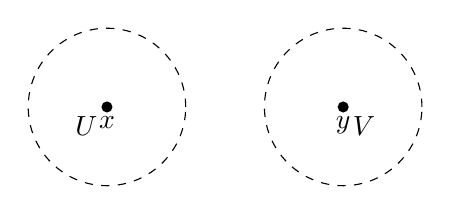
\begin{tikzpicture}
            % Draw the points x and y
            \fill (0,0) circle (2pt) node[below] {$x$};
            \fill (3,0) circle (2pt) node[below] {$y$};
    
            % Draw the open neighbourhoods U and V
            \draw[dashed] (0,0) circle (1) node[below left] {$U$};
            \draw[dashed] (3,0) circle (1) node[below right] {$V$};
        \end{tikzpicture}
        \caption{In a Hausdorff space, any two distinct points $x$ and $y$ can be separated by disjoint open neighbourhoods $U$ and $V$.}
        \label{lee-appendix-A.45D Hausdorff}
    \end{figure}
\end{itemize}





\begin{figure}[htbp]
    \centering
    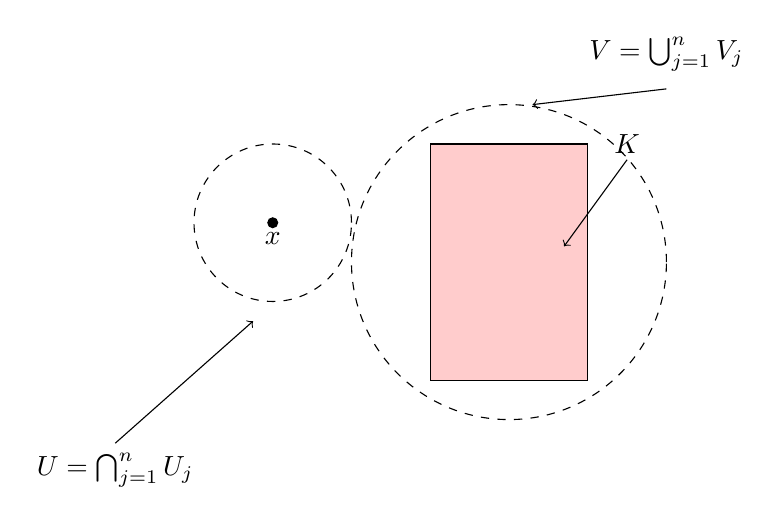
\begin{tikzpicture}
        % Draw the point x in A
        \fill (-0.5,0.5) circle (2pt);
        \node[below] at (-0.5,0.5) {$x$};
        
        % Draw the neighbourhood around x
        \draw[dashed] (-0.5,0.5) circle (1);
        \node[below] at (-2.5,-2.3) {$U=\bigcap_{j=1}^n U_j$};
        \draw[->] (-2.5,-2.3) -- (-0.75,-0.75);

        % Draw the closed set K
        \fill[red,opacity=0.2] (1.5,-1.5) rectangle (3.5,1.5);
        \draw (1.5,-1.5) rectangle (3.5,1.5);
        \node at (4,1.5) {$K$};
        \draw[->] (4,1.3) -- (3.2,0.2);

        % Draw the neighbourhood around K
        \draw[dashed] (2.5,0) circle (2);
        \node[above] at (4.5,2.3) {$V=\bigcup_{j=1}^n V_j$};
        \draw[->] (4.5,2.2) -- (2.8,2);
    \end{tikzpicture}
    \caption{Compact sets are closed in Hausdorff spaces}
    \label{lee-appendix-A.45D-compact-open}
\end{figure}

Let $V_y$ range through all possible $y\in K$, So that $\{V_y\}_{y\in K}$ is an open cover. There exists a finite subcollection of 'anchor points' of $K$, $y_1,\ldots,y_n$ that corresponds with $\{V_{y_j}\}_{j=1}^n$.

A finite intersection of open sets is again open, so 
\[
    U = \bigcap_{j=1}^n U_{y_j}\text{ is open }
\]
Define $V = \bigcup_{j=1}^nV_{y_j}$, so $V\subseteq K$ and $U\cap V = \varnothing$ and $x\in U\subseteq K^c$ (see \cref{lee-appendix-A.45D-compact-open}). Therefore $K$ is closed.\\



\begin{figure}[htbp]
    \centering
    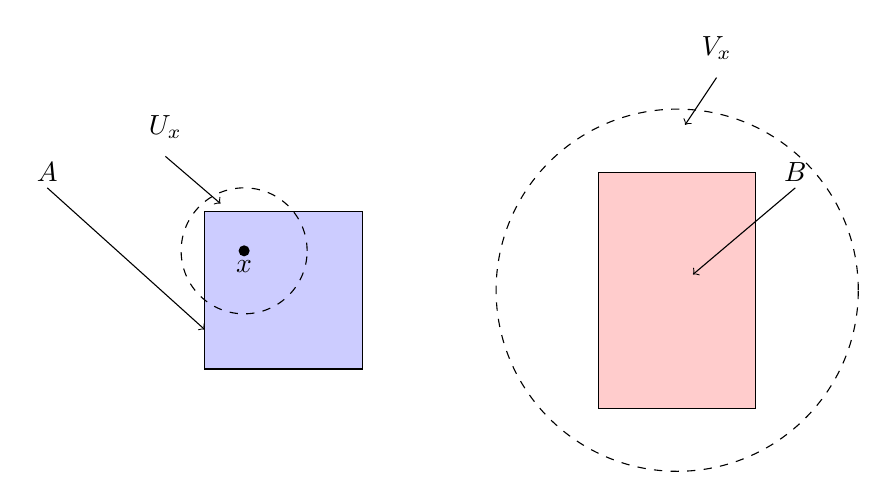
\begin{tikzpicture}
        % Draw the closed sets A and B
        \fill[blue,opacity=0.2] (-1,-1) rectangle (1,1);
        \draw (-1,-1) rectangle (1,1);
        \node at (-3,1.5) {$A$};
        \draw[->] (-3,1.3) -- (-1,-0.5);

        \fill[red,opacity=0.2] (4,-1.5) rectangle (6,1.5);
        \draw (4,-1.5) rectangle (6,1.5);
        \node at (6.5,1.5) {$B$};
        \draw[->] (6.5,1.3) -- (5.2,0.2);

        % Draw the point x in A
        \fill (-0.5,0.5) circle (2pt);
        \node[below] at (-0.5,0.5) {$x$};
        

        % Draw the neighbourhoods around x and B
        \draw[dashed] (-0.5,0.5) circle (0.8);
        \node[above] at (-1.5,1.8) {$U_x$};
        \draw[->] (-1.5,1.7) -- (-0.8,1.1);

        \draw[dashed] (5,0) circle (2.3);
        \node[above] at (5.5,2.8) {$V_x$};
        \draw[->] (5.5,2.7) -- (5.1,2.1);
    \end{tikzpicture}
    \caption{Closed sets $A$ and $B$, point $x$ in $A$, and disjoint neighbourhoods $U$ around $x$ and $V$ around $B$.}
    \label{lee-appendix-A.45D-closed-sets-separation}
\end{figure}

Finally, if $A$ and $B$ are disjoint compact sets, then each $x\in A\subseteq B^c$ induces neighbourhoods $x\in U_x$, and $B\subseteq V_x$ (see \cref{lee-appendix-A.45D-closed-sets-separation}), let $x$ range through all the elements of $A$. By compactness of $A$, this produces a finite subcover, and 

\[
    U = \bigcup_{j=1}^n U_{x_j}\quad V=\bigcap_{j=1}^n V_{x_j}
\]
are disjoint open sets that contain $A$ and $B$ respectively.





\end{proof}
\clearpage

\begin{proof}[Proof of \Cref{lee-appendix-A.45} Part E]
    Let $K\subseteq \xx$ be a closed set of a compact space. Let $\{U_\alpha\cap K\}$ be an open cover for $K$, where each $U_\alpha$ is open in $\xx$. We can append an extra set $K^c$ which is open in $\xx$. The collection

    \[
        W = \{U_\alpha\}\cup \{K^c\} \text{ covers }\xx
    \]
    so there exists a finite subcollection of $W_1,\ldots, W_n$ that cover $\xx$ (since $\xx$ is comapct by itself). Remove $K^c$ from this finite subcollection if it exists, and take the intersection with $K$ for each element $W_j$, and

    \[
        \{W_1\cap K,\ldots, W_n\cap K\} = \{U_1\cap K,\ldots, U_n\cap K\}\text{ covers }K
    \]
    so $K$ is compact.
\end{proof}
    
\begin{proof}[Proof of \Cref{lee-appendix-A.45} Part F]
    Proven in Part D.
\end{proof}
    
\begin{proof}[Proof of \Cref{lee-appendix-A.45} Part G]
    let $K\subseteq \xx$ be a compact subset of the metric space $(\xx,d)$. Compact subsets of $\xx$ are totally bounded, and hence bounded.
\end{proof}

\begin{proof}[Proof of \Cref{lee-appendix-A.45} Part H]
    See Tynchonoff's Theorem in Folland Chapter 4.
\end{proof}

\begin{proof}[Proof of \Cref{lee-appendix-A.45} Part I]
    Let $\xx$ and $\yy$ be topological spaces and $\pi: \xx\to\yy$ be a quotient map. So that $\yy$ is endowed with the quotient topology. So that $\pi$ is a surjective continuous map. and $\pi(\xx)=\yy$. Apply Part A, and we see that $\yy$ is compact.
\end{proof}

\end{document}

